\documentclass{article}

\usepackage[margin=0.8in]{geometry}
\usepackage{amsmath, amsfonts}
\usepackage{hyperref}
\usepackage{xcolor}
\usepackage{subcaption}
\usepackage{caption}
\usepackage{graphicx}

\setlength{\parindent}{0pt}

\begin{document}

\section*{Empirical convergence analysis}

\subsection*{Replay threshold}
The plots below show how the value of the root state changes with the EVB threshold $\xi$ at multiple horizons, 
inverse temperatures, and for various prior beliefs. Note that the root $Q$-values (i.e, the current MF $Q$-values) were set to $0$ 
everywhere, and the $Q$-values at all other belief states were set to the expected immediate reward.

\bigbreak

The prioritisation was determined by:

\begin{equation*}
    \text{EVB(b, a)} = p(b_{\rho}\rightarrow b, \pi) \times \mathbb{E}_{b' \sim p(b' \mid b, a, \pi)}\big[v(b')-v(b)\big]
\end{equation*}

where $b_{\rho}$ is the root belief and $\pi$ is a softmax policy.

\bigbreak

A couple of interesting observations. First, it looks like higher inverse temperature ($\beta$) needs 
fewer replays to approach the Bayes-optimal value at the root (it doesn't completely get there though 
because of the softmax). Second, there is an interesting horizon - $\xi$ trade-off -- higher horizons 
need fewer replays to get a better root value estimate than lower horizons; this means that one can 
(potentially) increase the horizon at the expense of setting a stricter (higher) $\xi$ threshold. As 
we have seen before, there is also a somewhat "emergent" depth-breadth trade-off which depends on 
uncertainty -- i.e., for the more uncertain arm the algorithm tends to backup values "in breadth", and 
for the more certain arm it goes more "in depth".  

\newpage

\begin{figure}[ht!]
    \centering
    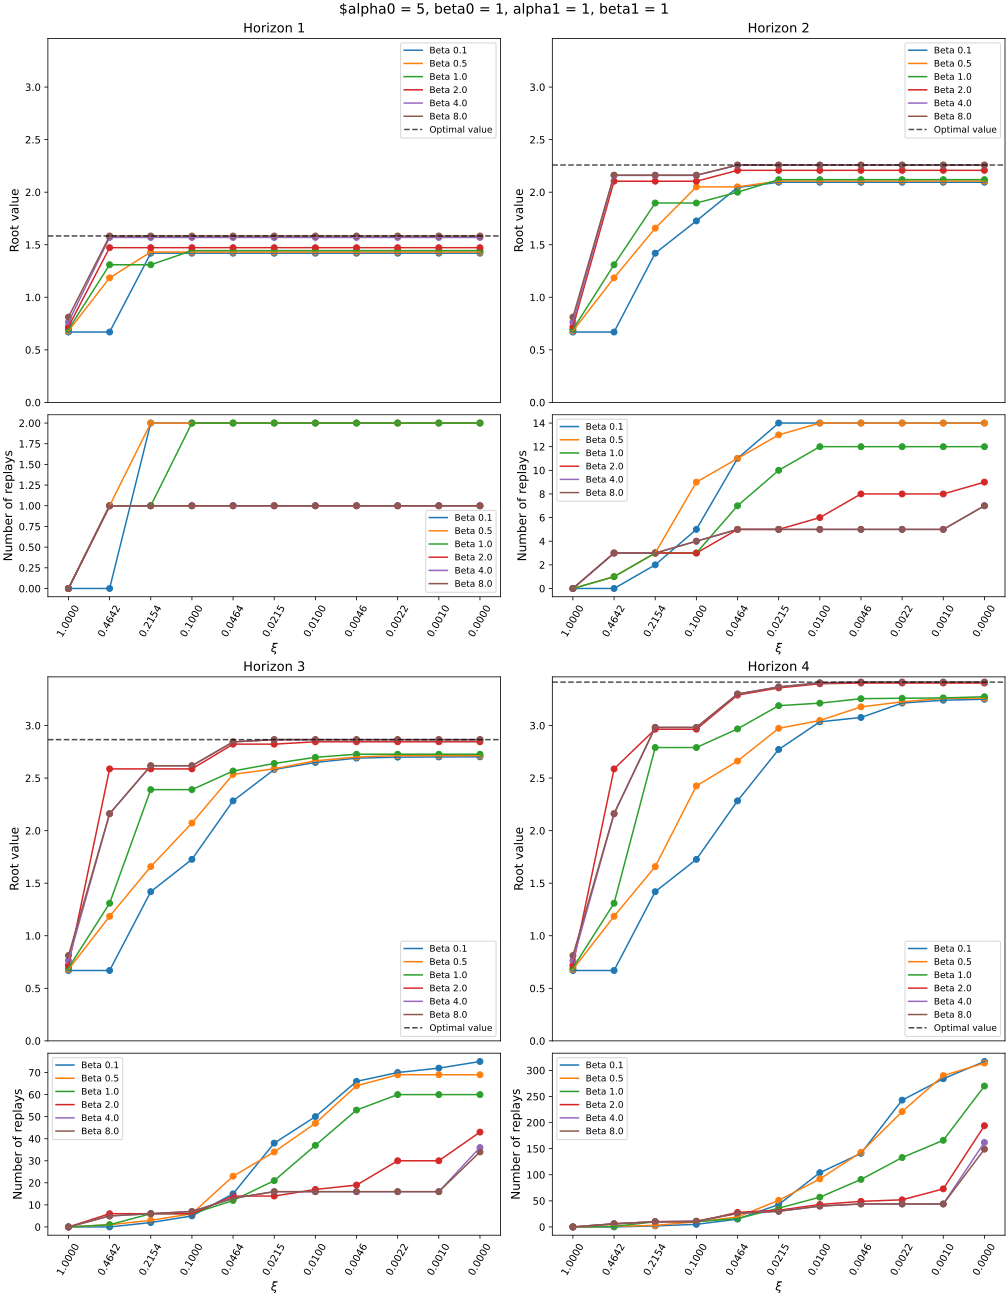
\includegraphics[width=1\textwidth]{../../../../bandit/data/convergence/xi/alpha05_beta01_alpha11_beta11_complete.png}
    \caption{Note that the same inverse temperature parameter $\beta$ was used within the tree and at the 
    root (which is the plotted root value).}
\end{figure}
\begin{figure}[ht!]
    \centering
    \includegraphics[width=1\textwidth]{../../../../bandit/data/convergence/xi/alpha05_beta02_alpha13_beta12_complete.png}
\end{figure}
\begin{figure}[ht!]
    \centering
    \includegraphics[width=1\textwidth]{../../../../bandit/data/convergence/xi/alpha09_beta06_alpha13_beta12_complete.png}
\end{figure}
\begin{figure}[ht!]
    \centering
    \includegraphics[width=1\textwidth]{../../../../bandit/data/convergence/xi/alpha010_beta06_alpha13_beta12_complete.png}
\end{figure}

\clearpage

\subsection*{Maze simulations}

The prioritisation of experiences at \textbf{distal} information states was detemined by:

\begin{equation*}
    \text{EVB}(<s, b>, a) = p(<s_{\rho}, b_{\rho}> \rightarrow <s, b>, \pi) \times \mathbb{E}_{<s', b'> \sim p(<s', b'> \mid <s, b>, a, \pi)}\big[v(<s', b'>)-v(<s,b>)\big]
\end{equation*}

where $s_{\rho}$ is the root physical state and $b_{\rho}$ is the root belief.

\bigbreak

The implementation is very similar to that of the bandit case -- during planning (replay), the agent generates a planning tree 
from every state and for every action. The updates can then happen either in distal parts of the trees (only 1 update is allowed 
at each iteration), or at the root. The value of each tree node is initialised to the agent's current MF $Q$-values.

\bigbreak

For the \textbf{root} action updates, the EVB is computed in the standard M\&D fashion:

\begin{equation*}
    \text{EVB}(<s_{\rho}, b_{\rho}>, a) = \text{Need}(<x, b_{\rho}> \rightarrow <s_{\rho}, b_{\rho}>, \pi) \times \text{Gain}(<s_{\rho}, b_{\rho}>, a)
\end{equation*}

This is a bit tricky to write down in a less cryptic way. Essentially, the assumption is that state 
$s_{\rho}$ can be reached from the agent's current location $x$ without belief dynamics -- that is, 
Need in this case is exactly the same as in M\&D.

\bigbreak

The crucial difference is the Gain term. Our Bayes-adaptive prioritised sweeping procedure effectively 
"chooses" which computation to perform at the root. Since it approximates a Bayes-optimal value (yet with 
a heuristic at the distal beliefs in the form of the current MF $Q$-values), the future information gain 
is subsumed by M\&D's Gain at the root.

\bigbreak

Below I show an example exploratory replay from a toy simulation. First, the agent was simulated in the 
environment for 3000 moves without being allowed to replay (so only MF learning) -- and luckily, with 
this seed, it never got to experience some of the bottom rightmost states (the ones where MF $Q$-values are 
all 0). The agent is completely certain 
about all transitions; however, at move 3000 I set its Beta posterior to $(1, 1)$ for the action 'up' below 
the rightmost barrier -- hence making it expect that the probability of that barrier being removed is $0.5$.
I then let it replay with horizon 2. The start state is the square which is the 3rd from the left at the very bottom. 

\bigbreak

The top left plots show MF $Q$-values and the agent's current location (green dot); the bottom left plots show 
the replay chosen by the agent; the top right plots show Gain; and the bottom right plots show Need. Note that 
only root updates are shown.

\newpage

\begin{figure}[ht!]
    \centering
    \includegraphics[width=1\textwidth]{../../../data/plots/move_3001.png}
\end{figure}
\begin{figure}[ht!]
    \centering
    \includegraphics[width=1\textwidth]{../../../data/plots/move_3001_0.png}
\end{figure}
\begin{figure}[ht!]
    \centering
    \includegraphics[width=1\textwidth]{../../../data/plots/move_3001_1.png}
\end{figure}
\begin{figure}[ht!]
    \centering
    \includegraphics[width=1\textwidth]{../../../data/plots/move_3001_2.png}
\end{figure}
\begin{figure}[ht!]
    \centering
    \includegraphics[width=1\textwidth]{../../../data/plots/move_3001_3.png}
\end{figure}
\begin{figure}[ht!]
    \centering
    \includegraphics[width=1\textwidth]{../../../data/plots/move_3001_4.png}
\end{figure}
\begin{figure}[ht!]
    \centering
    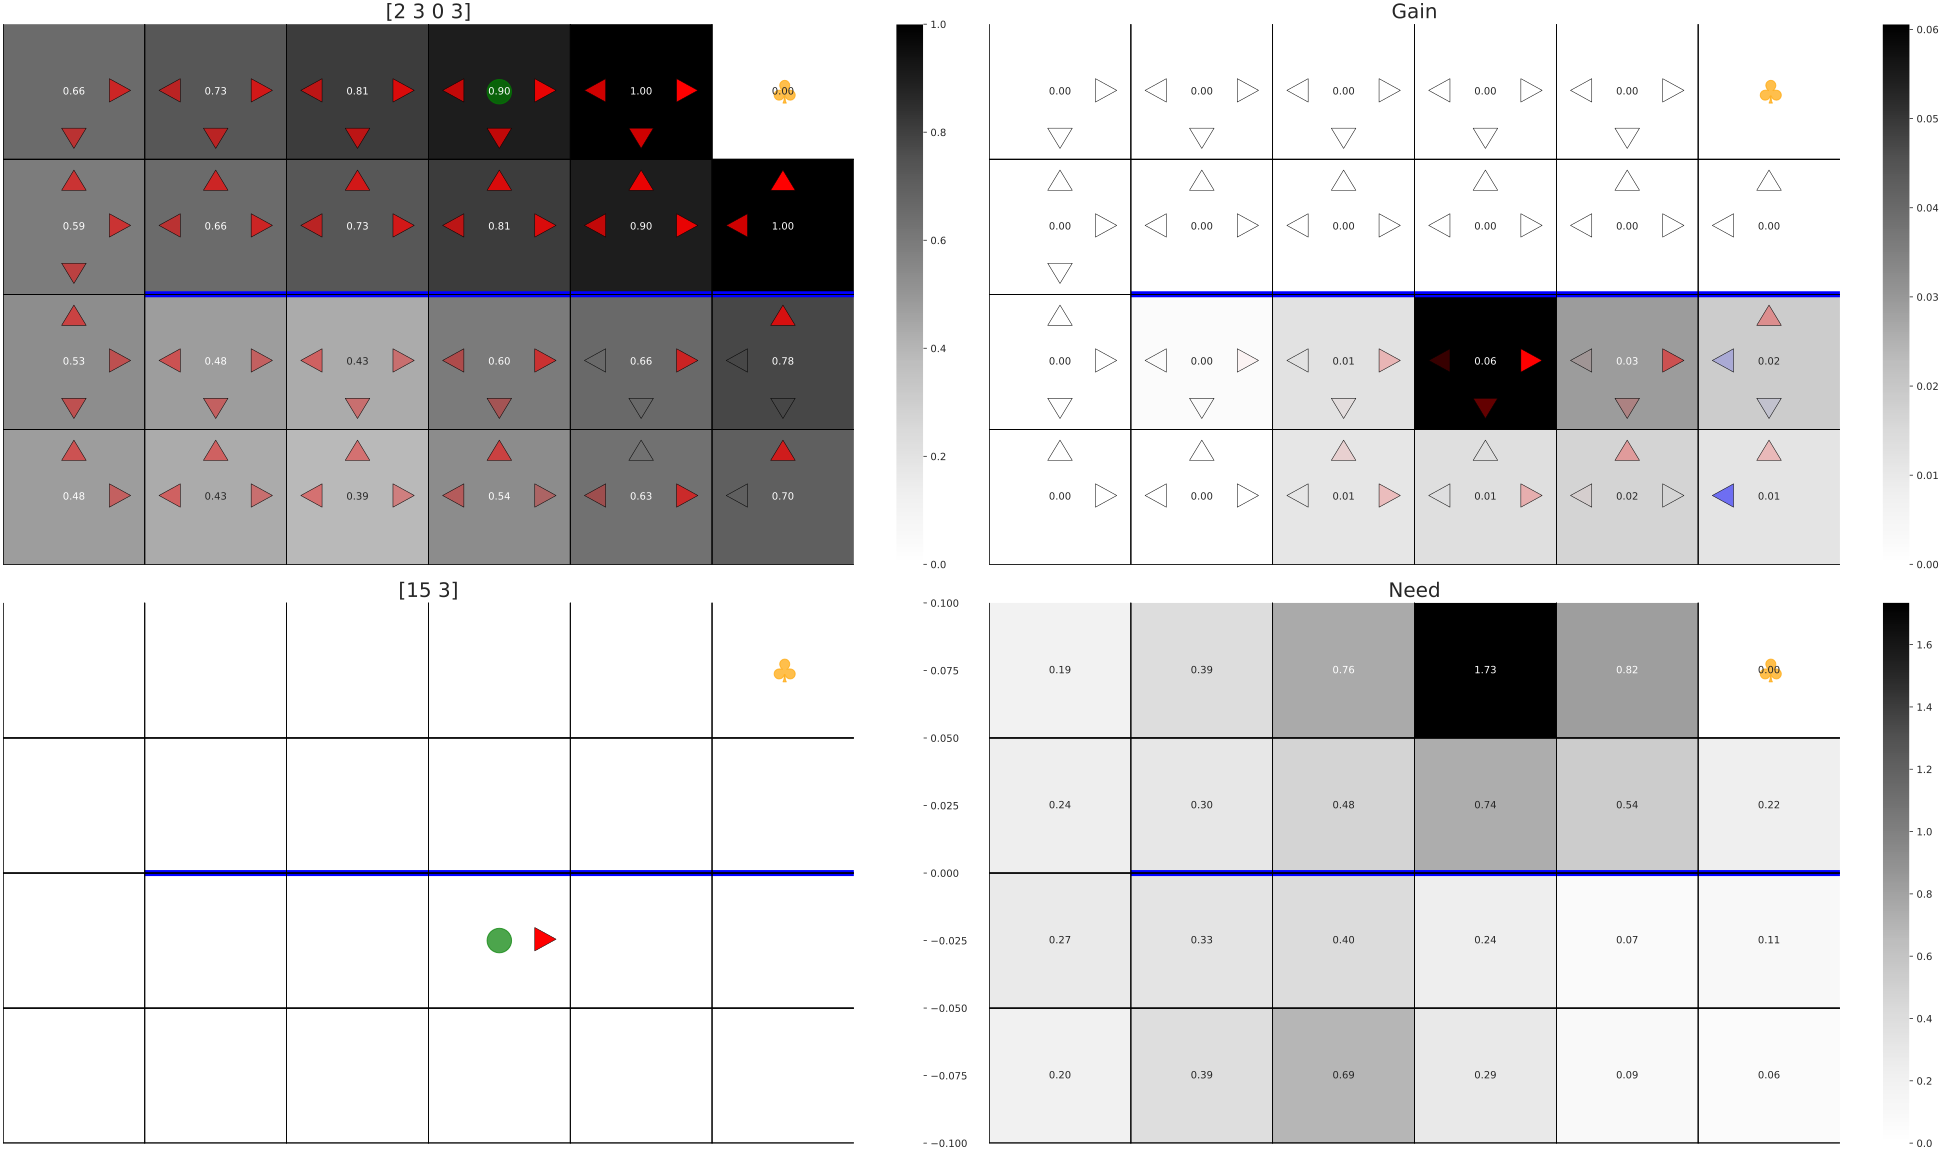
\includegraphics[width=1\textwidth]{../../../data/plots/move_3001_5.png}
\end{figure}

\clearpage

I think this is very interesting and there are quite a few important considerations here. First, the horizon really 
matters -- since it helps overcome the very low Need at (currenty) unexpected states. In the example shown above, 
for instance, if the horizon was set to 1, there would be no exploratory replays at all. This is because Need at the 
state adjacent to the shortcut is very small. However, for a larger horizon (2), the agent could plan crossing the 
barrier from a state which had a slightly higher Need -- just enough so that the expected value of that replay crossed 
the threshold, even though Gain was slightly lower due to $\gamma$ (which was set to $0.9$ in this simulation). That replay, in turn, 
increased the Need for the subsequent state (the one adjacent to the barrier), and hence that replay followed next. This 
is the reason why the model predicts such exploratory replays to proceed in a forward manner. 

\bigbreak

One thing which feels a bit uncomfortable is that Gain turns out to be much more powerful than Need (because Gain can dramatically change 
Need). This, of course, depends on the horizon and learning rates (replay learning rate was set to $1$ in this simulation), as well as 
the discount factor.

\bigbreak

For clarity, I also wrote down a very high-level pseudocode of the algorithm on the next page.

\newpage

\subsection*{Replay pseudocode}

\textbf{Initialise}\\ 
\begin{tabular}{ll}
    $x$ & $\leftarrow \text{agent's current physical state}$\\
    $b_{\rho}$ & $\leftarrow \text{agent's current belief}$ \\
    $H$ & $\leftarrow \text{horizon}$\\ 
    $\alpha_r$ & $\leftarrow \text{replay learning rate}$\\
    $\gamma$ & $\leftarrow \text{discount factor}$\\ 
    $\xi$ & $\leftarrow \text{EVB replay threshold}$  
\end{tabular}

\bigbreak

\textbf{for each} $s \in \mathcal{S}$ \textbf{do} \\
\hspace*{0.5cm} build belief tree $t_s$ with root information state $z_{\rho}=<s_{\rho}=s, b_{\rho}>$ up to horizon $H$\\
\hspace*{0.5cm} initialise $Q_{t_{s}(h)}(z=<k, b>, a) \leftarrow Q^{MF}(<k, b_{\rho}>, a) \; \; \forall h \in H, z \in t_{s}(h)$\\
\textbf{done}\\
\textbf{while} $\max_{z, a, t_{s}, h} \text{EVB}_{t_{s}(h)}(z, a) > \xi$ \textbf{do}\\
\hspace*{0.5cm} \textbf{for each} $h$ in $(H-1)$ \textbf{do}\\
\hspace*{0.5cm} \hspace*{0.5cm} \textbf{for each} information state $z=<k, b> \in t_s(h)$ \textbf{do}\\
\hspace*{0.5cm} \hspace*{0.5cm} \hspace*{0.5cm} \textbf{for each} action $a\in \mathcal{A}$ \textbf{do}\\
\hspace*{0.5cm} \hspace*{0.5cm} \hspace*{0.5cm} \hspace*{0.5cm} \textbf{if} $(h > 1)$ \textbf{do}\\
\hspace*{0.5cm} \hspace*{0.5cm} \hspace*{0.5cm} \hspace*{0.5cm} \hspace*{0.5cm} $\text{EVB}_{t_{s}(h)}(z, a) \leftarrow p(z_{\rho} \rightarrow z, \pi) \times \mathbb{E}_{z' \sim p(z' \mid z, a, \pi)}\big[v(z')-v(z)\big]$\\
\hspace*{0.5cm} \hspace*{0.5cm} \hspace*{0.5cm} \hspace*{0.5cm} \textbf{else if} $(h == 1)$ \textbf{do}\\
\hspace*{0.5cm} \hspace*{0.5cm} \hspace*{0.5cm} \hspace*{0.5cm} \hspace*{0.5cm} $\text{EVB}_{t_{s}(h)}(z_{\rho}, a) \leftarrow \text{Need}(<x, b_{\rho}> \rightarrow z_{\rho}, \pi) \times \text{Gain}(z_{\rho}, a)$\\
\hspace*{0.5cm} \hspace*{0.5cm} \hspace*{0.5cm} \hspace*{0.5cm} \textbf{done} \\
\hspace*{0.5cm} \hspace*{0.5cm} \hspace*{0.5cm} \textbf{done}\\
\hspace*{0.5cm} \hspace*{0.5cm} \textbf{done}\\
\hspace*{0.5cm} \textbf{done}\\
\hspace*{0.5cm} $z, a, t_s, h \leftarrow \text{argmax}_{z, a, t_{s}, h} \, \, \text{EVB}_{t_{s}(h)}(z, a)$\\
\hspace*{0.5cm} \textbf{if} $(h == 1)$ \textbf{do}\\
\hspace*{0.5cm} \hspace*{0.5cm} $Q^{MF}(z, a) \leftarrow Q_{t_{s}(h)}(z, a) + \alpha_r \mathbb{E}_{z'\sim p(z'\mid z, a, \pi)}\big[R(z') + \gamma \max_{a' \in \mathcal{A}}Q_{t_{s}(h+1)}(z', a') - Q(z, a)_{t_s(h)}\big]$\\
\hspace*{0.5cm} \hspace*{0.5cm} \textbf{for each} $s \in \mathcal{S}$ \textbf{do} \\
\hspace*{0.5cm} \hspace*{0.5cm} \hspace*{0.5cm} build belief tree $t_s$ with root information state $z_{\rho}=<s_{\rho}=s, b_{\rho}>$ up to horizon $H$\\
\hspace*{0.5cm} \hspace*{0.5cm} \hspace*{0.5cm} initialise $Q_{t_{s}(h)}(z=<k, b>, a) \leftarrow Q^{MF}(<k, b_{\rho}>, a) \; \; \forall h \in H, z \in t_{s}(h)$\\
\hspace*{0.5cm} \hspace*{0.5cm} \textbf{done}\\
\hspace*{0.5cm} \textbf{else if} $(h != 1)$ \textbf{do}\\
\hspace*{0.5cm} \hspace*{0.5cm} $Q_{t_{s}(h)}(z, a) \leftarrow Q_{t_{s}(h)}(z, a) + \alpha_r \mathbb{E}_{z'\sim p(z'\mid z, a, \pi)}\big[R(z') + \gamma \max_{a' \in \mathcal{A}}Q_{t_{s}(h+1)}(z', a') - Q(z, a)_{t_s(h)}\big]$\\
\hspace*{0.5cm} \textbf{done}\\
\textbf{repeat}



\end{document}
